\section{Factory-Muster}
\subsection{Problemstellung} Einfach
\begin{itemize}
\item Man moechte eine Pizzeria mit mehreren Zweigstellen erstellen.
\item Bei der Zubereitung der Pizza gibt diverse Arbeitsablaeufe die von den Zweigstellen allesamt 
  unterschiedliche abgearbeitet werden koennen (Z.B. Schneiden: Vierteln vs. in acht Stuecke 
  schneiden, etc.).
\item` Problem: Um Code-Dopplung zu vermeiden sollen die Pizza in einer einzigen Klasse implementiert 
  sein -> Es muss ein Pizza-Objekt entsprechend den Anforderungen (welche Zweigstelle?) erstellt 
  werden. 
\end{itemize}
  
\subsection{Loesung}
Es wird eine abstrakte Superklasse \emph{Pizzeria} erstellt. Verschiedene Zweigstellen beerben diese. 
Jede dieser Zweigstellen implementiert eine Methode \emph{erstellePizza()}. Diese dient als so 
genannte Factory, denn sie erstellt ein Objekt des gew"unschten Typs. Bei der Erstellung wird ein 
entsprechender Konstruktor einer speziellen Pizza-Klasse aufgerufen. Diese Klasse implementiert 
die Methoden der Arbeitsschritte (backen, schneiden, etc.) entsprechend. In der Superklasse wird 
eine Methode deklariert ("bestellePizza()") die mit diesem Objekt arbeitet. Durch den 
Polymorphismus / Abstraktion ist es irrelevant mit welchem Pizza-Objekt man arbeitet, da alle 
erbenden Klassen des Pizza-Typs die dort aufgerufenen Methoden implementiert / geerbt haben. Die 
Methode "bestellePizza()" wird auch fabrikMethode genannt.



\subsection{Problemstellung: Erweitert}
\begin{itemize}
\item Einzelne Zweigstellen benutzen minderwertige Zutaten.
\item Wie kann man man Konsistenz bei den Zutaten sichern?
\end{itemize}

\subsection{Loesung}
\todo{noch unbearbeitet}



\begin{figure}
	\centering
	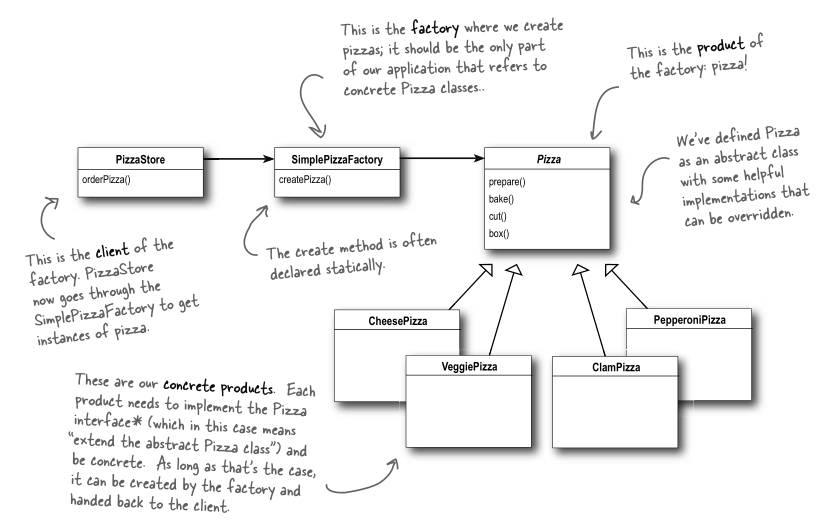
\includegraphics[width=\linewidth]{factory/img/simpleFactoryUML}
	\caption{UML-Darstellung des \emph{einfachen} Factory-Musters}
	\label{fig:simpleFactoryUML}
\end{figure}
